\chapter{Approach}
\label{chap:approach}

\section{Overview}
\label{sec:overview}

\begin{figure}
    \centering
    \rotatebox{0}{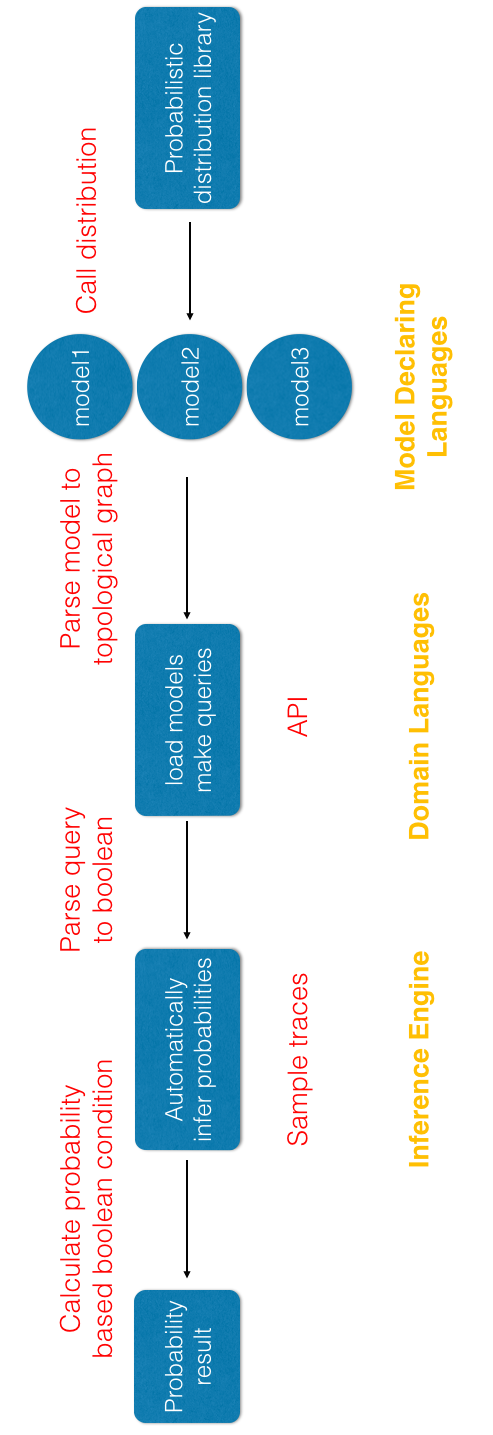
\includegraphics[width=0.5\textwidth]{figures/overview.png}}
    \caption{Overview of the Portable Probabilistic Programming Framework.}
    \label{fig:overview}
\end{figure}

The structure of the framework is showed in Figure ~\ref{fig:overview}. Users can define probabilistic models in our model declaring language, where they can directly call the functions of distributions without implementing the distributions. They can load the models and write queries in their domain languages with the APIs. Then the inference engine will infer the queries automatically based on the sampling traces. Thus the desired probability will be derived.

There are four steps in the design and implementation of the portable probabilistic programming framework. At first we designed the syntax of the embedded programming language, which targets the description of the Bayesian networks. The design of the language is based on BUGS, but the syntax is more specific and efficient to be lightweight for the portable characteristic. Also the syntax can be expressive for most of the probabilistic models. The description of the models using the portable probabilistic programming language is separated from the code of the host language as well of the conditional query, which can enhance the reusability of the probabilistic models. The parser is implemented and the inference engine is generated automatically based on the conditional query. More details will be illustrated in Section ~\ref{sec:syntax}. 

We implemented the probabilistic library for most of the probability distribution such as Gaussian, Gama, Beta, etc. Our probabilistic programs define distributions by defining a distribution over possible execution traces. The distribution is fully specified by a generative procedure. More details can be found in Section ~\ref{sec:distr}. 

The inference algorithm is based on the MCMC sampling, including rejection sampling and Metropolis-Hastings Algorithm, which is efficient and lightweight to implement. We will elaborate more on the mechanism of the inference engine in Section ~\ref{sec:infer}. 

Additionally, we implement the APIs for other languages leveraging the existing development tool: SWIG (Simplified Wrapper and Interface Generator). More details for the APIs are in Section ~\ref{sec:api}.

Our main contribution lies in the design of the portable probabilistic programming language to make it portable, the implementation of the probability distribution library and the lightweight implementation of the inference engine.


\section{Syntax of Programming Language}
\label{sec:syntax}
We will give some intuition of our portable probabilistic programming language by giving an example declaring the flip model, which is showed in Figure ~\ref{fig:flip_eg}. 

\begin{figure}
    \centering
    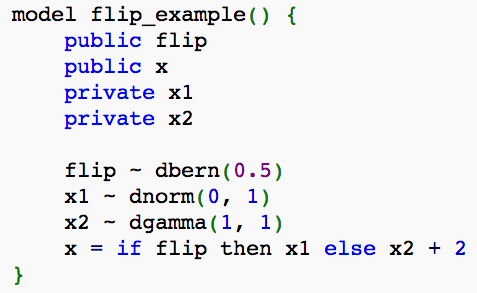
\includegraphics[width=0.6\textwidth]{figures/flip_eg.png}
    \caption{Flip example, describing the probabilistic model in our language.}
    \label{fig:flip_eg}
\end{figure}

The flip example describes a probabilistic model that has the distribution over variables as showed in Figure ~\ref{fig:flip_dist}. The grammar for this specific example is showed in Figure ~\ref{fig:flip_syn}. Under this syntax, the parser will parse the probabilistic program and generate the Bayesian network as the user described. The inference is done based on the probabilistic graph. The Bayesian network of the flip example is showed in Figure ~\ref{fig:flip_net}.


\begin{figure}
    \centering
    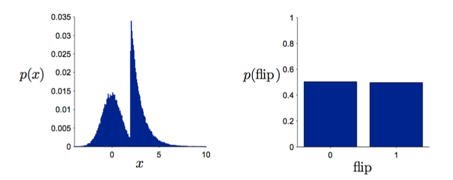
\includegraphics[width=0.8\textwidth]{figures/flip_dist.png}
    \caption{Flip example, the implied distributions over variables.}
    \label{fig:flip_dist}
\end{figure}

\begin{figure}
    \centering
    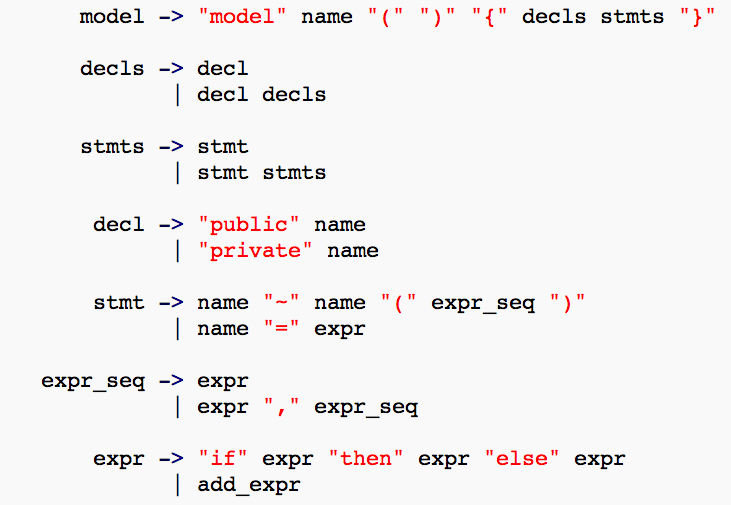
\includegraphics[width=0.7\textwidth]{figures/flip_syn.png}
    \caption{The grammar for the flip example.}
    \label{fig:flip_syn}
\end{figure}


\begin{figure}
    \centering
    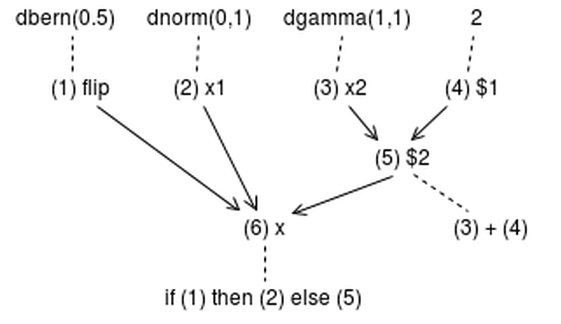
\includegraphics[width=0.6\textwidth]{figures/flip_net.png}
    \caption{The generated Bayesian network for the flip example.}
    \label{fig:flip_net}
\end{figure}

The grammar for the portable probabilistic programming language is as below:
\begin{align*}
           models \rightarrow & ~model \\
                   |& ~model ~models \\       
            model \rightarrow & ~\textcolor{red}{``model"} ~name \textcolor{red}{``("}~~~~~~~~~~~~~~~~~ \textcolor{red}{``)"} ~ \textcolor{red}{``\{"} decls ~stmts \textcolor{red}{``\}"} \\
                   |& ~\textcolor{red}{``model"} name \textcolor{red}{``("} model\_params \textcolor{red}{``)"} ~\textcolor{red}{``\{"} decls ~stmts \textcolor{red}{``\}"} \\         
     model\_params \rightarrow & ~name \\
                   |& ~name ~\textcolor{red}{``,"}~ model\_params \\        
            decls \rightarrow & ~decl \\
                   |& ~decl ~decls \\ 
            stmts \rightarrow & ~stmt \\
                   |& ~stmt ~stmts \\        
             decl \rightarrow & ~\textcolor{red}{``public"} ~variable \\
                   |& ~\textcolor{red}{``private"} ~variable \\         
             stmt \rightarrow & ~variable ~\textcolor{red}{``\sim"} ~name ~\textcolor{red}{``("} ~expr\_seq ~\textcolor{red}{``)"} \\
                   |& ~variable ~\textcolor{red}{``="} ~expr \\
                   |& ~\textcolor{red}{``for"} ~name ~\textcolor{red}{``="} ~expr ~\textcolor{red}{``to"} ~expr ~\textcolor{red}{``\{"} stmts \textcolor{red}{``\}"} \\        
         expr\_seq \rightarrow & ~expr \\
                   |& ~expr ~\textcolor{red}{``,"} ~expr\_seq \\      
\end{align*}

\begin{align*}   
             expr \rightarrow & ~\textcolor{red}{``if"} ~expr ~\textcolor{red}{``then"} ~expr ~\textcolor{red}{``else"} ~expr \\
                   |& ~\textcolor{red}{``new"} ~name ~\textcolor{red}{``("} ~\textcolor{red}{``)"} \\
                   |& ~add\_expr \\  
         add\_expr \rightarrow & ~term \\
                   |& ~term ~\textcolor{red}{``+"} ~add\_expr \\
                   |& ~term ~\textcolor{red}{``-"} ~add\_expr            
             term \rightarrow & ~primary \\  
                   |& ~primary \textcolor{red}{``*"} ~term \\
                   |& ~primary \textcolor{red}{``/"} ~term \\
          primary \rightarrow & ~numerical\_value \\
                   |& ~variable \\
                   |& ~function\_call \\
                   |& ~\textcolor{red}{``("} ~expr ~\textcolor{red}{``)"} \\
                   |& ~\textcolor{red}{``-"} ~primary \\           
    function\_call \rightarrow & ~name ~\textcolor{red}{``("} ~expr\_seq ~\textcolor{red}{``)"} \\           
         variable \rightarrow & ~name \\
                   |& ~field\_var \\
                   |& ~index\_var \\              
        field\_var \rightarrow & ~name ~\textcolor{red}{``."} ~name \\
        index\_var \rightarrow & ~name ~\textcolor{red}{``["} ~expr\_seq ~\textcolor{red}{``]"} \\           
  numerical\_value \rightarrow & ~integer\_value \\
                   |& ~integer\_value ~\textcolor{red}{``."} ~integer\_value \\                  
    integer\_value \rightarrow & ~[0-9]+ \\            
             name \rightarrow & ~[a-zA-Z\_][0-9a-zA-Z\_]*
\end{align*}

Users can declare many probabilistic graphical models in our declarative programming language. Figure ~\ref{fig:hmm} shows an example of Hidden Markov Model(HMM) described in our language and Figure ~\ref{fig:ldacode} shows an example of Latent Dirichlet Allocation(LDA).

\begin{figure}
  \begin{lstlisting}[language=C]
    model hidden_markov_model(n, a, b) {
        // n -- chain length
        // a -- number of possible states
        // b -- number of possible observations
        public states[n]   // hidden states
        public observ[n]   // observations
        public trans[a,a]  // transition matrix of size a*a
        public emiss[a,b]  // emission matrix of size a*b
        public start[a]    // start probabilities of size a

        states[0] ~ dcat(start)
        for i = 1 to n-1 {
            states[i] ~ dcat(trans[states[i-1]])
        }

        for i = 0 to n-1 {
            observ[i] ~ dcat(emiss[states[i]])
        }
    }
  \end{lstlisting}
  \caption{An HMM example}
  \label{fig:hmm}
\end{figure}

\begin{figure}
  \begin{lstlisting}[language=C]
    model latent_dirichlet_allocation(k, num_docs, num_words[], vocab_size) {
      for i = 1 to k {
        topics(i, :) = dirichlet(1, vocab_size);
      }
      
      for i = 1 to num_docs {
        topic_dist = dirichlet(1, k);
        for j = 1 to num_words(i) {
          topic = multinomial(topic_dist);
          X{i}(j) = multinomial(topics(topic, :));
        }
      }
    }
  \end{lstlisting}
  \caption{An LDA example}
  \label{fig:ldacode}
\end{figure}

In our design, the declarations of the Bayesian networks and the query of conditional probability is seperated. Users can describe the model in a model file and load the model in their domain languages. In this way, users can reuse their models and load several probabilistic graphical models at the same time. Also their queries can base on these models which have a better structure than mixing the models up. Examples of writing the queries and load models can be found in ~\ref{sec:api}.

\section{Probabilistic Distribution Library}
\label{sec:distr}
We implemented the probabilistic library for most of the probability distribution such as Gaussian, Gama, Beta, etc. Our probabilistic programs define distributions by defining a distribution over possible execution traces. The distribution is fully specified by a generative procedure. Some complex distributions are crafted compositionally. An example is showed on how to implement a Gaussian Mixture Model distribution in Figure ~\ref{fig:gmm}. As can be seen in Figure ~\ref{fig:gmm}., everytime we run the function $gmm()$, it will return a value based on the distribution implementation. And the trace of the returned value will meet the requirements of the density probability the program has defined.

\begin{figure}
    \centering
    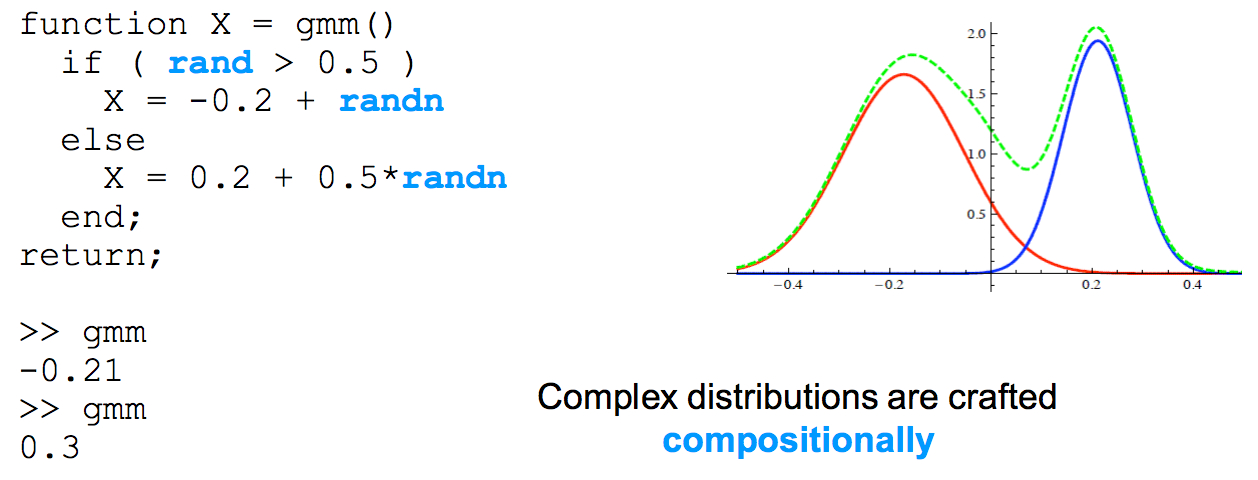
\includegraphics[width=0.9\textwidth]{figures/gmm.png}
    \caption{Implementation of GMM distribution example.}
    \label{fig:gmm}
\end{figure}

Most of the distributions in our library are implemented based on Normal distribution and Bernoulli distribution according to mathematical algorithms. The probability distributions in our framework contain:

\begin{center}
\begin{tabular}{|l|l|}
  \hline
  Code & Distribution \\
  \hline
  dbern & Bernoulli distribution \\
  dnorm & Normal distribution \\
  dgamma & Gamma distribution \\ 
  dbinomial & Binomial distribution \\
  dmultinomial & Multinomial distribution \\
  ddirich & Dirichlet distribution\\
  dbeta & Beta distribution \\
  duniform & Uniform distribution \\
  duniform\_discrete & Discrete uniform distribution \\
  dpoisson & Poisson distribution \\
  dcat & Categorical distribution \\
  \hline
\end{tabular}
\end{center}

There are many algorithms to generate values from some specific probability distribution. For example, to generate values from Gaussian distribution, there is Box-Muller transform method ~\cite{box} and Ziggurat algorithm ~\cite{ziggurat}. We leveraged Ziggurat algorithm in our framework since it is faster and still exact. 

\begin{figure}
    \centering
    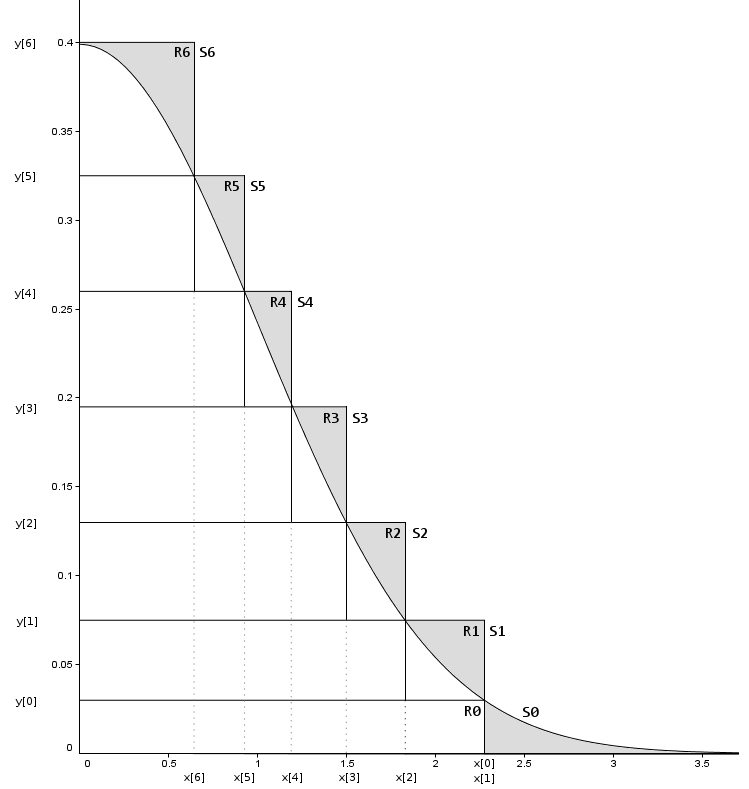
\includegraphics[width=0.7\textwidth]{figures/ziggurat.png}
    \caption{The ziggurat method with 7 rectangles.}
    \label{fig:ziggurat}
\end{figure}

As is showed in Figure ~\ref{fig:ziggurat}, each rectangular is a layer. Given uniform random variables $U_0,~U_1 \in [0,1)$, the ziggurat algorithm can be described as:
\begin{enumerate}
  \item Choose a random layer $0 \leq i < n$.
  \item Let $x = U_0 \times x_i$
  \item If $x < x_i + 1$, return $x$.
  \item If $i == 0$, generate a point from the tail using the fallback algorithm.
  \item Let $y = y_i + U_1 \times (y_i + 1 - y_i)$.
  \item Compute $f(x)$. If $y < f(x)$, return $x$.
  \item Otherwise, choose new random numbers and go back to step 1.
\end{enumerate}

\section{Inference Engine}
\label{sec:infer}
Calculating the distribution specified by a probabilistic program is called \textit{probabilistic inference}. The inferred probability distribution is called the \textit{posterior probability distribution}, and the initial guess made by the program is called the \textit{prior probability distribution}. Let $(E; F)$ be a partitioning of the node indices of a graphical model into disjoint subsets, such that $(X_E, X_F)$ is a partitioning of the random variables. There are two kinds of inference problems that we want to solve:
\begin{itemize}
  \item Marginal probabilities:
  \begin{align*}
    p(x_E) = \sum_{x_F} p(x_E, x_F).
  \end{align*}
  \item Maximum a posteriori(MAP) probabilities:
  \begin{align*}
    p^*(x_E) = max_{x_F} ~p(x_E, x_F).
  \end{align*}
\end{itemize}
From these basic computations we can obtain other quantities of interest. In particular, the \textit{conditional probability} $p(x_E | x_F)$ is equal to
\begin{align*}
  p(x_E | x_F) = \frac{p(x_E, x_F)}{\sum_{x_E} p(x_E, x_F)}.
\end{align*}

The mechanism of our inference engine is based on sampling. Currently we used Rejection Sampling algorithm in the inference engine, which is straightforward and easy to implement. However, rejection Sampling is not as efficient as other sampling algorithms like Gibbs Sampling and Metropolis-Hastings algorithm. Henceforth, we added another optional inference algorithm in our inference engine: Metropolis-Hastings algorithm. 

There are three problems we need to consider in stochastic sampling:
\begin{itemize}
  \item how to generate samples
  \item how to incorporate observations
  \item how to infer probabilities from samples
\end{itemize}
The intuitive idea is to sample the traces as the program runs. If the trace meets the Boolean requirements of the condition, then record the trace, otherwise the trace is discarded. Then we calculate the number of the traces that can meet the Boolean requirement of the probability we want to get. Then calculating this number over the whole number of traces we recorded can derive the final conditional probability.

\subsection{Rejection Sampling}
\textit{Rejection sampling} is a basic technique used to generate observations from a distribution. It is a type of Monte Carlo method. The method works for any distribution in $\mathbb{R}^m$ with a density.

\begin{figure}
    \centering
    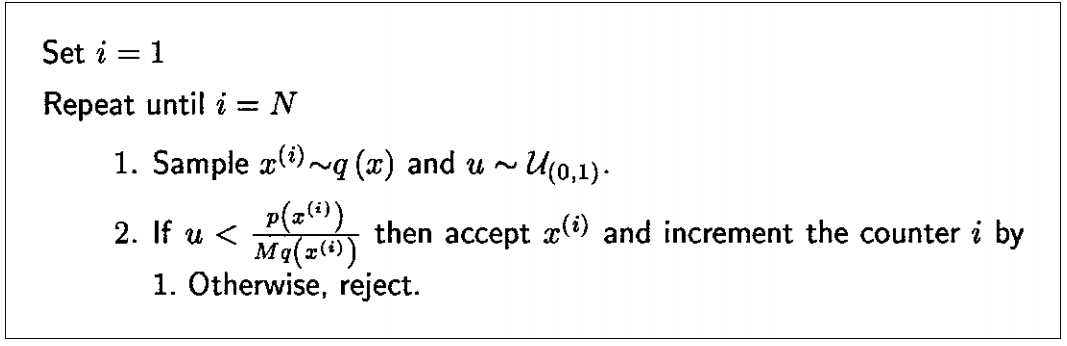
\includegraphics[width=0.9\textwidth]{figures/rj1.png}
    \caption{Rejection sampling algorithm. Here, $u \sim \mathscr{U}(0,1)$ denotes the operation of sampling a uniform random variable on the interval $(0,1)$.}
    \label{fig:rj1}
\end{figure}

\begin{figure}
    \centering
    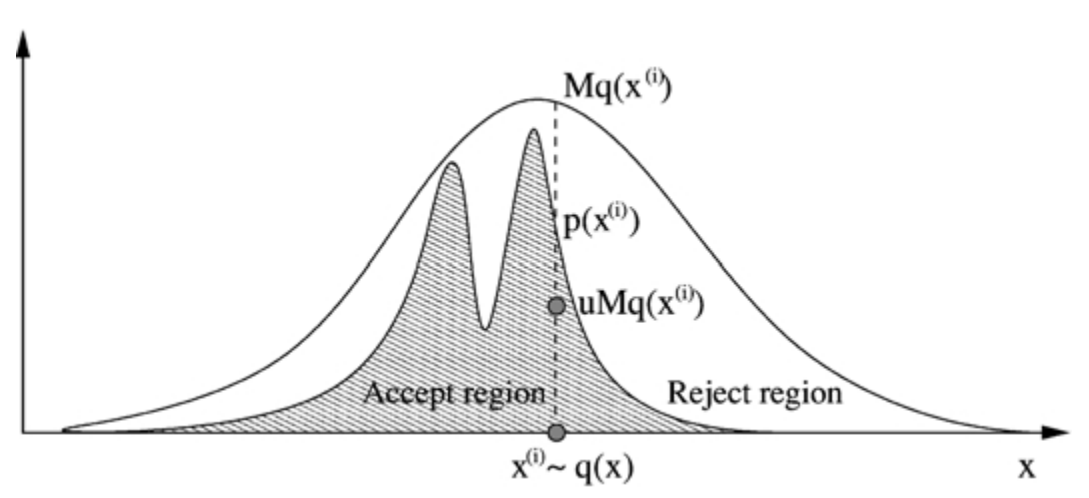
\includegraphics[width=0.7\textwidth]{figures/rj2.png}
    \caption{Rejection sampling: Sample a candidate $x(i)$ and a uniform variable $u$. Accept the candidate sample if $uMq(x^{(i)}) < p(x^{(i)})$, otherwise reject it.}
    \label{fig:rj2}
\end{figure}

Rejection sampling is based on the observation that to sample a random variable one can sample uniformly from the region under the graph of its density function. We can sample from a distribution $p(x)$, which is known up to a proportionality constant, by sampling from another easy-to-sample proposal distribution $q(x)$ that satisfies $p(x) \leq Mq(x), M < \infty$, using the accept/reject procedure describe in Figure ~\ref{fig:rj1} (see also Figure ~\ref{fig:rj2}). ~\cite{mcmc}
The accepted $x(i)$ can be easily shown to be sampled with probability $p(x)$ ~\cite{robert}. This simple method suffers from severe limitations. It is not always
possible to bound $p(x) \/ q(x)$ with a reasonable constant $M$ over the whole space $X$. If $M$ is too large, the acceptance probability 
\begin{align*}
  Pr(x ~ accepted) = Pr(u < \frac{p(x)}{Mq(x)}) = \frac{1}{M}
\end{align*}
will be too small. This makes the method impractical in high-dimensional scenarios.

\subsection{Metropolis-Hastings Algorithm}

\begin{figure}
    \centering
    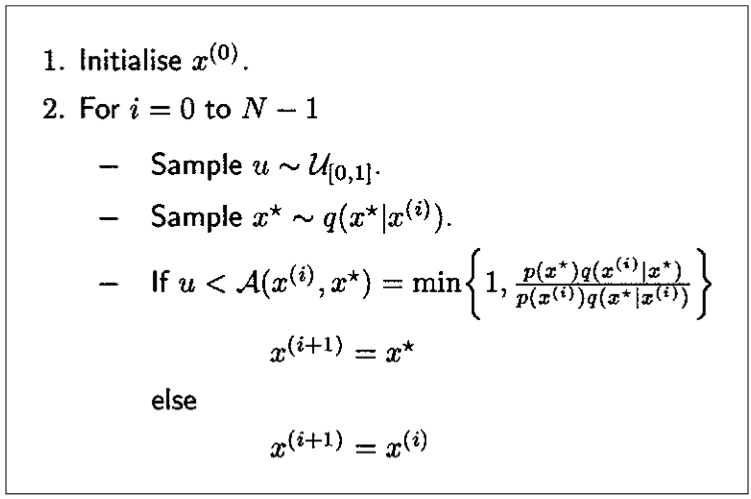
\includegraphics[width=0.7\textwidth]{figures/mh.png}
    \caption{Metropolis-Hastings algorithm.}
    \label{fig:mh}
\end{figure}

\begin{figure}
    \centering
    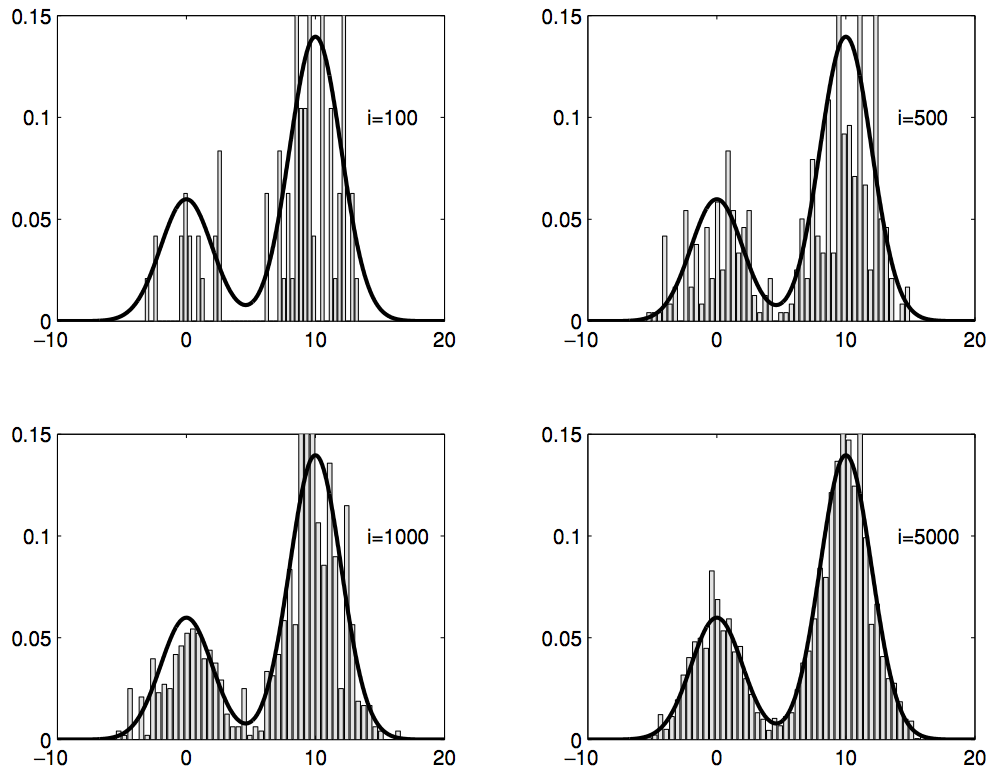
\includegraphics[width=0.7\textwidth]{figures/mh2.png}
    \caption{Target distribution and histogram of the MCMC samples at different iteration points.}
    \label{fig:mh2}
\end{figure}

The \textit{Metropolis-Hastings (MH) algorithm} is the most popular MCMC method. An MH step of invariant distribution $p(x)$ and proposal distribution $q(x^*	| x)$ involves sampling a candidate value $x^*$ given the current value $x$ according to $q(x^* | x)$. The Markov chain then moves towards $x^*$ with acceptance probability
\begin{align*}
  \mathscr{A}(x, x^*) = min\{1,\frac{p(x^*)q(x | x^*)}{p(x)q(x^* | x)} \}
\end{align*}
otherwise it remains at $x$. The pseudo-code is shown in Figure ~\ref{fig:mh}, while Figure ~\ref{fig:mh2} shows the results of running the MH algorithm with a Gaussian proposal distribution
\begin{align*}
  q(x^* | x(i)) = Normal(x^{(i)}, 100)
\end{align*}
and a bimodal target distribution
\begin{align*}
  p(x) \propto 0.3 \times exp(−0.2x^2) + 0.7 exp(−0.2{(x - 10)}^2)
\end{align*}
for 5000 iterations. As expected, the histogram of the samples approximates the target distribution.

The MH algorithm is very simple, but it requires careful design of the proposal distribution $q(x^* | x)$. In general, it is possible to use suboptimal inference and learning algorithms to generate data-driven proposal distributions.

The transition kernel for the MH algorithm is
\begin{align*}
  K_{MH}(x^{(i + 1)} | x^{(i)}) = q(x^{(i + 1)} | x^{(i)}) \mathscr{A}(x^{(i)}, x^{(i + 1)}) + \sigma_{x^{(i)}} (x^{(i + 1)}) r (x^{(i)}),
\end{align*}  
where $r(x^{(i)})$ is the term associated with rejection
\begin{align*}
  r(x^{(i)}) = \int_{\chi} q(x^* | x^{(i)})(1 - \mathscr{A}(x^{(i)}), x^*)dx^*
\end{align*}
It is fairly easy to prove that the samples generated by MH algorithm will mimic samples
drawn from the target distribution asymptotically. By construction, $K_{MH}$ satisfies the detailed
balance condition
\begin{align*}
  p(x^{(i)})K_{MH}(x^{(i + 1)} | x^{(i)}) = p(x^{(i + 1)})K_{MH}(x^{(i)} | x^{(i + 1)})
\end{align*}
and, consequently, the MH algorithm admits $p(x)$ as invariant distribution. To show that the MH algorithm converges, we need to ensure that there are no cycles (aperiodicity)
and that every state that has positive probability can be reached in a finite number of steps (irreducibility). Since the algorithm always allows for rejection, it follows that it is aperiodic. To ensure irreducibility, we simply need to make sure that the support of $q(\cdotp)$ includes the support of $p(\cdotp)$.

The independent sampler and the Metropolis algorithm are two simple instances of the MH algorithm. In the independent sampler the proposal is independent of the current state, $q(x^* | x^{(i)}) = q(x^*)$. Hence, the acceptance probability is
\begin{align*}
  \mathscr{A}(x^{(i)} | x^*) = min \{1, \frac{p(x^*)q(x^{(i)})}{p(x^{(i)})q(x^*)}\}
\end{align*}
The Metropolis algorithm assumes a symmetric random walk proposal $q(x^* | x^{(i)}) = q(x^{(i)} | x^*)$ and, hence, the acceptance ratio simplifies to
\begin{align*}
  \mathscr{A}(x^{(i)}, x^*) = min \{ 1, \frac{p(x^*)}{p(x^{(i)})} \}
\end{align*}

\subsection{From Samples to Probabilities}
We can get traces of samples after the sampling algorithm. Probabilities can be estimated from a set of examples using the sample average. The sample average of a proposition $\alpha$ is the number of samples where $\alpha$ is true divided by the total number of samples. The sample average approaches the true probability as the number of samples approaches infinity by the law of large numbers.

We treat the condtion and the desired posterior as booleans. We will take a very simple query as example to illustrate how to calculate probability after sampling. Given a query
\begin{align*}
  P (X = 1| Y < 2)
\end{align*}
we will get traces of samples where the samples all meet the condition $Y < 2$. The number of such samples generated is $n$. There are some other samples generated in the sampling process that can not meet the boolean requirement, which we will not count them in $n$. Then from these left $n$ samples, we may find $t$ samples that also meet the boolean requirement of $X = 1$. Thus the desired conditional probability would be $t / n$.

\section{APIs for Other Languages}
\label{sec:api}
We leveraged the development tool SWIG (Simplified Wrapper and Interface Generator) ~\cite{swig} to make other languages be able to call for C functions, as we implemented the framework in C. SWIG is an interface compiler that connects programs written in C and C++ with scripting languages such as Perl, Python, Ruby, and Tcl. It works by taking the declarations found in C/C++ header files and using them to generate the wrapper code that scripting languages need to access the underlying C/C++ code. Once the user has the APIs, users are able to call the load probabilistic model function and inference function in each common language. That's how the portable is implemented. 

The supported languages is listed as below:

\begin{center}
\begin{tabular}{|l|l|l|}
\hline
Tcl & Python & Perl \\
\hline
Guile & Java & Ruby \\
\hline
Mzscheme & PHP & OCaml \\
\hline
C\# & Pike & Chincken Scheme \\
\hline
Allegro CL & Modula-3 & Lua \\
\hline
Lisp & R & Octave \\
\hline
Go & D & Javascript \\
\hline
\end{tabular}
\end{center}

No matter what domain languages we choose to use, the language to describe the probabilistic graphical model is the same, whose concrete syntax is showed in programming language syntax section, in Section ~\ref{sec:syntax}. Below is an example to declare the flip model in our declaration language:

\begin{lstlisting}[language=C]
  model flip_example() {
      public flip
      public x
      private x1
      private x2

      flip ~ dbern(0.5)
      x1 ~ dnorm(0, 1)
      x2 ~ dgamma(1, 1)
      x = if flip then x1 else x2 + 2
  }
\end{lstlisting}

The challenge in this part is the C/C++ pointer doesn’t exist in other languages like Java and Python. We cope with this problem by using wrapper with a specific form to hint the difference of the pointers and the normal variables.
  
We will give some examples of how our framework can be used in other common language like \textbf{C, Python, Java}.
  
\subsection{C API}
To encode the previous flip example in C, the APIs is showed as following:
\begin{lstlisting}[language=C]
#include <stdio.h>
#include "ppp.h"
#include <stdlib.h>
#include <time.h>

int main()
  {
      /* use pointers to structs because the client doesn't need to know the struct sizes */
      struct pp_state_t* state;
      struct pp_instance_t* instance;
      struct pp_query_t* query;
      struct pp_trace_store_t* traces;
      float result;

      srand(time(NULL));
      state = pp_new_state();
      printf("> state created\n");

      pp_load_file(state, "parse/models/flip.model");
      printf("> file loaded\n");

      instance = pp_new_instance(state, "flip_example", 0);
      printf("> instance created\n");

      query = pp_compile_query(instance, "x>2, x<3");
      printf("> condition compiled\n");

      traces = pp_sample(instance, query);
      printf("> traces sampled\n");

      query = pp_compile_query(instance, "flip==1");
      printf("> query compiled\n");

      pp_get_result(traces, query, &result);  /* "get_result" may not be a good name */
      printf("%f\n", result);

      pp_infer(instance, "flip == 1", "x > 2, x < 3", &result);  /* alternative way to get a result */
      printf("%f\n", result);

      pp_free(state);  /* free memory, associated models, instances, queries, and trace stores are deallocated */

      return 0;
  }
\end{lstlisting}
  
\subsection{Python API}
If we want to encode the flip example in the same way in Python, we need to add an interface file which is the input to SWIG. The $swig$ command produces a file ``example\_wrap.c" that should be compiled and linked with the rest of the program. In this case, we have built a dynamically loadable extension that can be loaded into the Python interpreter using the `load' command. The interface file is showed in Figure ~\ref{fig:ifile}.

\begin{figure}[h]
\begin{lstlisting}[language=C]
  /* libppp.i */
  %module libppp
  %include "typemaps.i"
  %apply float *OUTPUT { float * result };
  %{
  /* Put header files here or function declarations like below */
  #include "libppp.h"
  %}

  %include "libppp.h"
\end{lstlisting}
\caption{Interface file}
\label{fig:ifile}
\end{figure}
where ``\texttt{libppp.h}'' is the original c header file containing the public APIs for user to load the model and make quiries, which is showed in Figure ~\ref{fig:libppp}.

\begin{figure}[h]
\begin{lstlisting}[language=C]
  struct pp_state_t;
  struct pp_instance_t;
  struct pp_query_t;
  struct pp_trace_store_t;
 
  struct pp_state_t* pp_new_state();
  int pp_free(struct pp_state_t* state);
 
  int pp_load_file(struct pp_state_t* state, const char* filename);
  struct pp_instance_t* pp_new_instance(struct pp_state_t* state, const char* model_name, int* model_params);
 
  struct pp_query_t* pp_compile_query(struct pp_instance_t* instance, const char* query_string);
  struct pp_trace_store_t* pp_sample(struct pp_instance_t* instance, struct pp_query_t* query);
  int pp_get_result(struct pp_trace_store_t* traces, struct pp_query_t* query, float* result);
 
  // P(X|Y)
  int pp_infer(struct pp_instance_t* instance, const char* X, const char* Y, float* result);
\end{lstlisting}
\caption{Header file of public APIs}
\label{fig:libppp}
\end{figure}

And the API usage in Python in showed in Figure ~\ref{fig:python}.

\begin{figure}
\begin{lstlisting}[language=Python]
import libppp

state = libppp.pp_new_state()

libppp.pp_load_file(state, "../parse/models/flip.model")

instance = libppp.pp_new_instance(state, "flip_example", None)

query = libppp.pp_compile_query(instance, "x>2, x<3")

traces = libppp.pp_sample(instance, query)

query = libppp.pp_compile_query(instance, "flip==1")

success, result = libppp.pp_get_result(traces, query)
print("success:", success, "result:", result)

success, result = libppp.pp_infer(instance, "flip == 1", "x > 2, x < 3")
print("success:", success, "result:", result)

libppp.pp_free(state); 
\end{lstlisting}
\caption{Python API usage example}
\label{fig:python}
\end{figure}

\subsection{Java API}
\begin{figure}
\begin{lstlisting}[language=Java]
public class Flip {
    public static void main(String[] args) {
        System.setProperty("java.library.path", ".");
        System.loadLibrary("libppp");
        SWIGTYPE_p_pp_state_t state = libppp.pp_new_state();
        SWIGTYPE_p_pp_instance_t instance;
        SWIGTYPE_p_pp_query_t query;
        SWIGTYPE_p_pp_trace_store_t traces;
        int success;
        float[] result = new float[2];

        libppp.pp_load_file(state, "../parse/models/flip.model");

        instance = libppp.pp_new_instance(state, "flip_example", null);

        query = libppp.pp_compile_query(instance, "x>2, x<3");

        traces = libppp.pp_sample(instance, query);

        query = libppp.pp_compile_query(instance, "flip==1");

        success = libppp.pp_get_result(traces, query, result);
        System.out.printf("result: d%", result);

        success = libppp.pp_infer(instance, "flip == 1", "x > 2, x < 3", result);
        System.out.printf("result: d%", result);

        libppp.pp_free(state);
    }
}
\end{lstlisting}
\caption{Java API usage example}
\label{fig:java}
\end{figure}

Similarly, a Java version for the flip example can be seen in Figure ~\ref{fig:java}.\\

\subsection{Ocaml API}
If we want to use the model in Ocaml, we can use the API as showed in Figure ~\ref{fig:ocaml}. \\

\begin{figure}
  \begin{lstlisting}[language=Caml]
    open libppp

    let flip_eg =
      let state = Libppp.pp_new_state() in

      Libppp.pp_load_file(state, "../parse/models/flip.model")

      let instance = Libppp.pp_new_instance(state, "flip_example", None) in

      let query = Libppp.pp_compile_query(instance, "x>2, x<3") in

      let traces = Libppp.pp_sample(instance, query) in

      let query = Libppp.pp_compile_query(instance, "flip==1") in

      let (success, result) = Libppp.pp_get_result(traces, query) in

      let (success, result) = Libppp.pp_infer(instance, "flip == 1", "x > 2, x < 3") in

      Libppp.pp_free(state);
  \end{lstlisting}
  \caption{Ocaml API usage example}
  \label{fig:ocaml}
\end{figure}

For other languages, the APIs are similar. The interface file is just used to encode the public APIs of the framework and it is only used once to generate the wrapper of APIs in other languages. So users do not need to write the interface file on their own. They can directly write the queries in domain languages and load models in model files.
